\documentclass[10pt,a4paper]{article}
\usepackage[paper=a4paper, left=1.5cm, right=1.5cm, bottom=2.0cm, top=1.6cm]{geometry}
\usepackage[utf8]{inputenc} % para poder usar tildes en archivos UTF-8
\usepackage[spanish]{babel} % para que comandos como \today den el resultado en castellano
\usepackage[conEntregas]{caratula}
\usepackage{amsmath}
\usepackage[colorlinks=true, linkcolor=blue]{hyperref}
\usepackage[section]{placeins}

\usepackage{ifpdf}
\usepackage{multicol}
\usepackage{caption}
\usepackage{subcaption}
\usepackage{listings}
\usepackage{float}

\begin{document}

\titulo{Trabajo Práctico 2}
\subtitulo{Rutas en Internet}

\fecha{\today}

\materia{Teoría de las comunicaciones}

%\grupo{Grupo ?}

\integrante{Interlandi, Daniel}{773/00}{danielinterlandi@yahoo.com.ar}
\integrante{Ladelfa, Hern\'an Nahuel}{318/04}{nahueladelfa@gmail.com}

\maketitle
\tableofcontents
\pagebreak
  
\section{Resúmen}

El objetivo de este trabajo es el de experimentar con las herramientas provistas por el protocolo ICMP para analizar las rutas tomadas por los paquetes hasta alcanzar su destino. Además se analizará la existencia de saltos entre nodos intercontinentales en las rutas de los experimentos.

\section{Introducción}

\section{Implementación}

Para este trabajo implementamos nuestra propia versión de la herramienta \texttt{traceroute}, en lenguaje \emph{Python} y utilizando la librería \emph{Scapy}.
\\
El funcionamiento de nuestro programa es similar al del \texttt{traceroute} que se encuentra en los sistemas operativos más conocidos. Para lograr encontrar la ruta que podrían seguir los paquetes para alcanzar a un host destino lo que hacemos es ir enviando paquetes \emph{ICMP Echo Request}, comenzando con un valor de TTL (Time To Live) igual a uno e incrementando este valor gradualmente. De esta forma, cada router al recibir estos paquetes decrementará el valor del TTL en uno. Si, luego de decrementar el valor del TTL, el mismo queda en cero, el router que posee el paquete responderá al host origen con un mensaje \emph{ICMP Time Exceeded}. Cuando un paquete alcanza finalmente al host destino, este responderá con un mensaje \emph{ICMP Echo Reply}. De esta forma, recibiendo los sucesivos mensajes \emph{ICMP Time Exceeded} de cada router y con el mensaje final \emph{ICMP Echo Reply}, podremos armar una ruta con los routers intermedios hasta el host destino.
\\
Para evitar que el programa nunca finalize por intentar alcanzar al destino cuando este no responde, agregamos una cota al valor del TTL de 40.
También, para cada valor de TTL realizamos hasta 10 intentos para encontrar la ruta. De esta forma podría darse la situación en que encontremos más de una ruta posible. Por lo tanto, si obtenemos al menos 3 veces consecutivas respuesta del mismo nodo, lo tomamos como parte de la ruta que retornaremos como respuesta y su RTT (Roundtrip Time) será el promedio de sus muestras.
\\\\
Además, a este programa le agregamos los cálculos necesarios para encontrar los enlaces entre nodos cuyos valores de RTT se encuentran considerablemente por encima del resto. Es decir, que buscaremos encontrar los outliers de las muestras. Estos cálculos los utilizaremos para inferir cuáles son los enlaces intercontinentales. Para encontrar a estos outliers utilizaremos la técnica de estimación de John M. Cimbala propuesta por la cátedra. Veremos más detalles sobre estos cálculos en la siguiente sección.
\\\\
Para utilizar nuestra versión de \texttt{traceroute} se debe ejecutar:

\begin{lstlisting}[language=bash]
  $ python traceroute.py <host> 
\end{lstlisting}

Donde:

\begin{itemize}
\item host: Es la dirección IP o nombre de dominio del host destino hasta el cual se quiere calcular la ruta.
\end{itemize}
\pagebreak
\section{Estimación de outliers}

Basándonos en la técnica de estimación propuesta por John M. Cimbala para encontrar los outliers de una muestra, agregamos a nuestro programa los cálculos necesarios para inferir saltos intercontinentales en las rutas tomadas por los paquetes hacia un host destino.
\\\\
Los pasos que seguiremos para realizar estos cálculos fueron:

\begin{enumerate}
\item 
Para cada TTL de los \emph{ICMP Echo Request} enviados, a partir del RTT medido, calculamos el dRTT (delta RTT) de cada salto entre cada par de nodos como:
\[
\\dRTT_i =RTT_i - RTT_{i-1}
\]

Donde $RTT_i$ es el valor de RTT en cada paso. 

\item
Debido a que \texttt{traceroute} no es una herramienta del todo precisa, los resultados pueden presentar ciertas anomalías que se manifiestan con resultados extraños o erróneos. Uno de estos comportamientos podría darse cuando, para un valor de TTL el paquete \emph{ICMP Echo Reply} toma un camino más largo que el paquete \emph{ICMP Echo Reply} correspondiente al TTL siguiente. En este caso, el RTT del primero terminará siendo mayor que el siguiente, logrando que el dRTT de este último tome un valor negativo. Esto nunca podría ocurrir en la realidad, ya que el tiempo que tarda un paquete en llegar de un nodo a otro más lejano siempre debería ser positivo.
\\
Para salvar este comportamiento indeseado y evitar que la búsqueda de outliers se vea afectada, decidimos reemplazar a todos los dRTT negativos por el valor del promedio de todos los dRTT positivos obtenidos. De esta forma buscamos que estos dRTT incorrectos se acerquen más a valores reales. 

\item
Utilizamos al conjunto de los $dRTT_i$ como los valores de nuestra muestra, con $i=1,…,n$. Donde $n$ es la cantidad de muestras obtenidas.
Ordenamos la muestra de forma creciente.

\item
Por cada $dRTT_i$ calculamos el valor absoluto del desvío como:
\[
\delta_i = |dRTT_i - \overline{dRTT}|
\]

Donde $\overline{dRTT}$ es el valor de la media de la muestra calculado como el promedio de los $dRTT_i$ medidos.

\item
Tomamos como referencia la tabla de valores calculados para la fórmula de \emph{Thompson modificada} del artículo de Cimbala para obtener el valor $\tau$ correspondiente a las $n$ muestras. Con este valor obtuvimos:
\[
\tau S = \tau * S
\]

Donde S es el desvío estándar calculado como:
\[
S=\sqrt{\frac{\sum_{i=1}^{n} (dRTT_i - \overline{dRTT})^2}{n-1}}
\]

\item
Luego, tomamos el último valor (el máximo) de la muestra ordenada y verificamos, si se cumple que $\delta_i > \tau S$, entonces se asume que el salto con $dRTT_i$ es un enlace intercontinental. Removemos este $dRTT_i$ de la muestra y volvemos a intentar con el nuevo último valor de la muestra hasta que no se cumpla la desigualdad mencionada anteriormente, donde habremos terminado de encontrar los outliers.
\end{enumerate}

De esta forma, mediante una técnica estadística y las herramientas que brinda el protocolo \emph{ICMP}, logramos inferir cuáles son los enlaces intercontinentales en las rutas tomadas por los paquetes.
\pagebreak
\section{Resultados}

\subsection{Segunda Consigna: Gráficos y Análisis}

\subsubsection{Red Doméstica}

Para la primera captura, se eligió una red domestica de uno de los integrantes del grupo. Los dispositivos conectados a la red en este caso fueron, 3 computadoras, 2 celulares, un televisor SmartTV y un Apple TV. Todos estos conectados al modem del proveedor de internet.
La captura duró aproximadamente 30 minutos.
Al ser una red pequeña podemos distinguir fácilmente los nodos destacados.
La Figura~\ref{fig:red_domestica_network}. muestra 2 nodos destacados. 192.168.0.1 que corresponde al router  y el nodo 192.168.0.27 correspondiente al SmartTV que en el momento de la captura de los paquetes, el mismo se encontraba actualizandose.

\begin{figure}[h!]
  \centering
   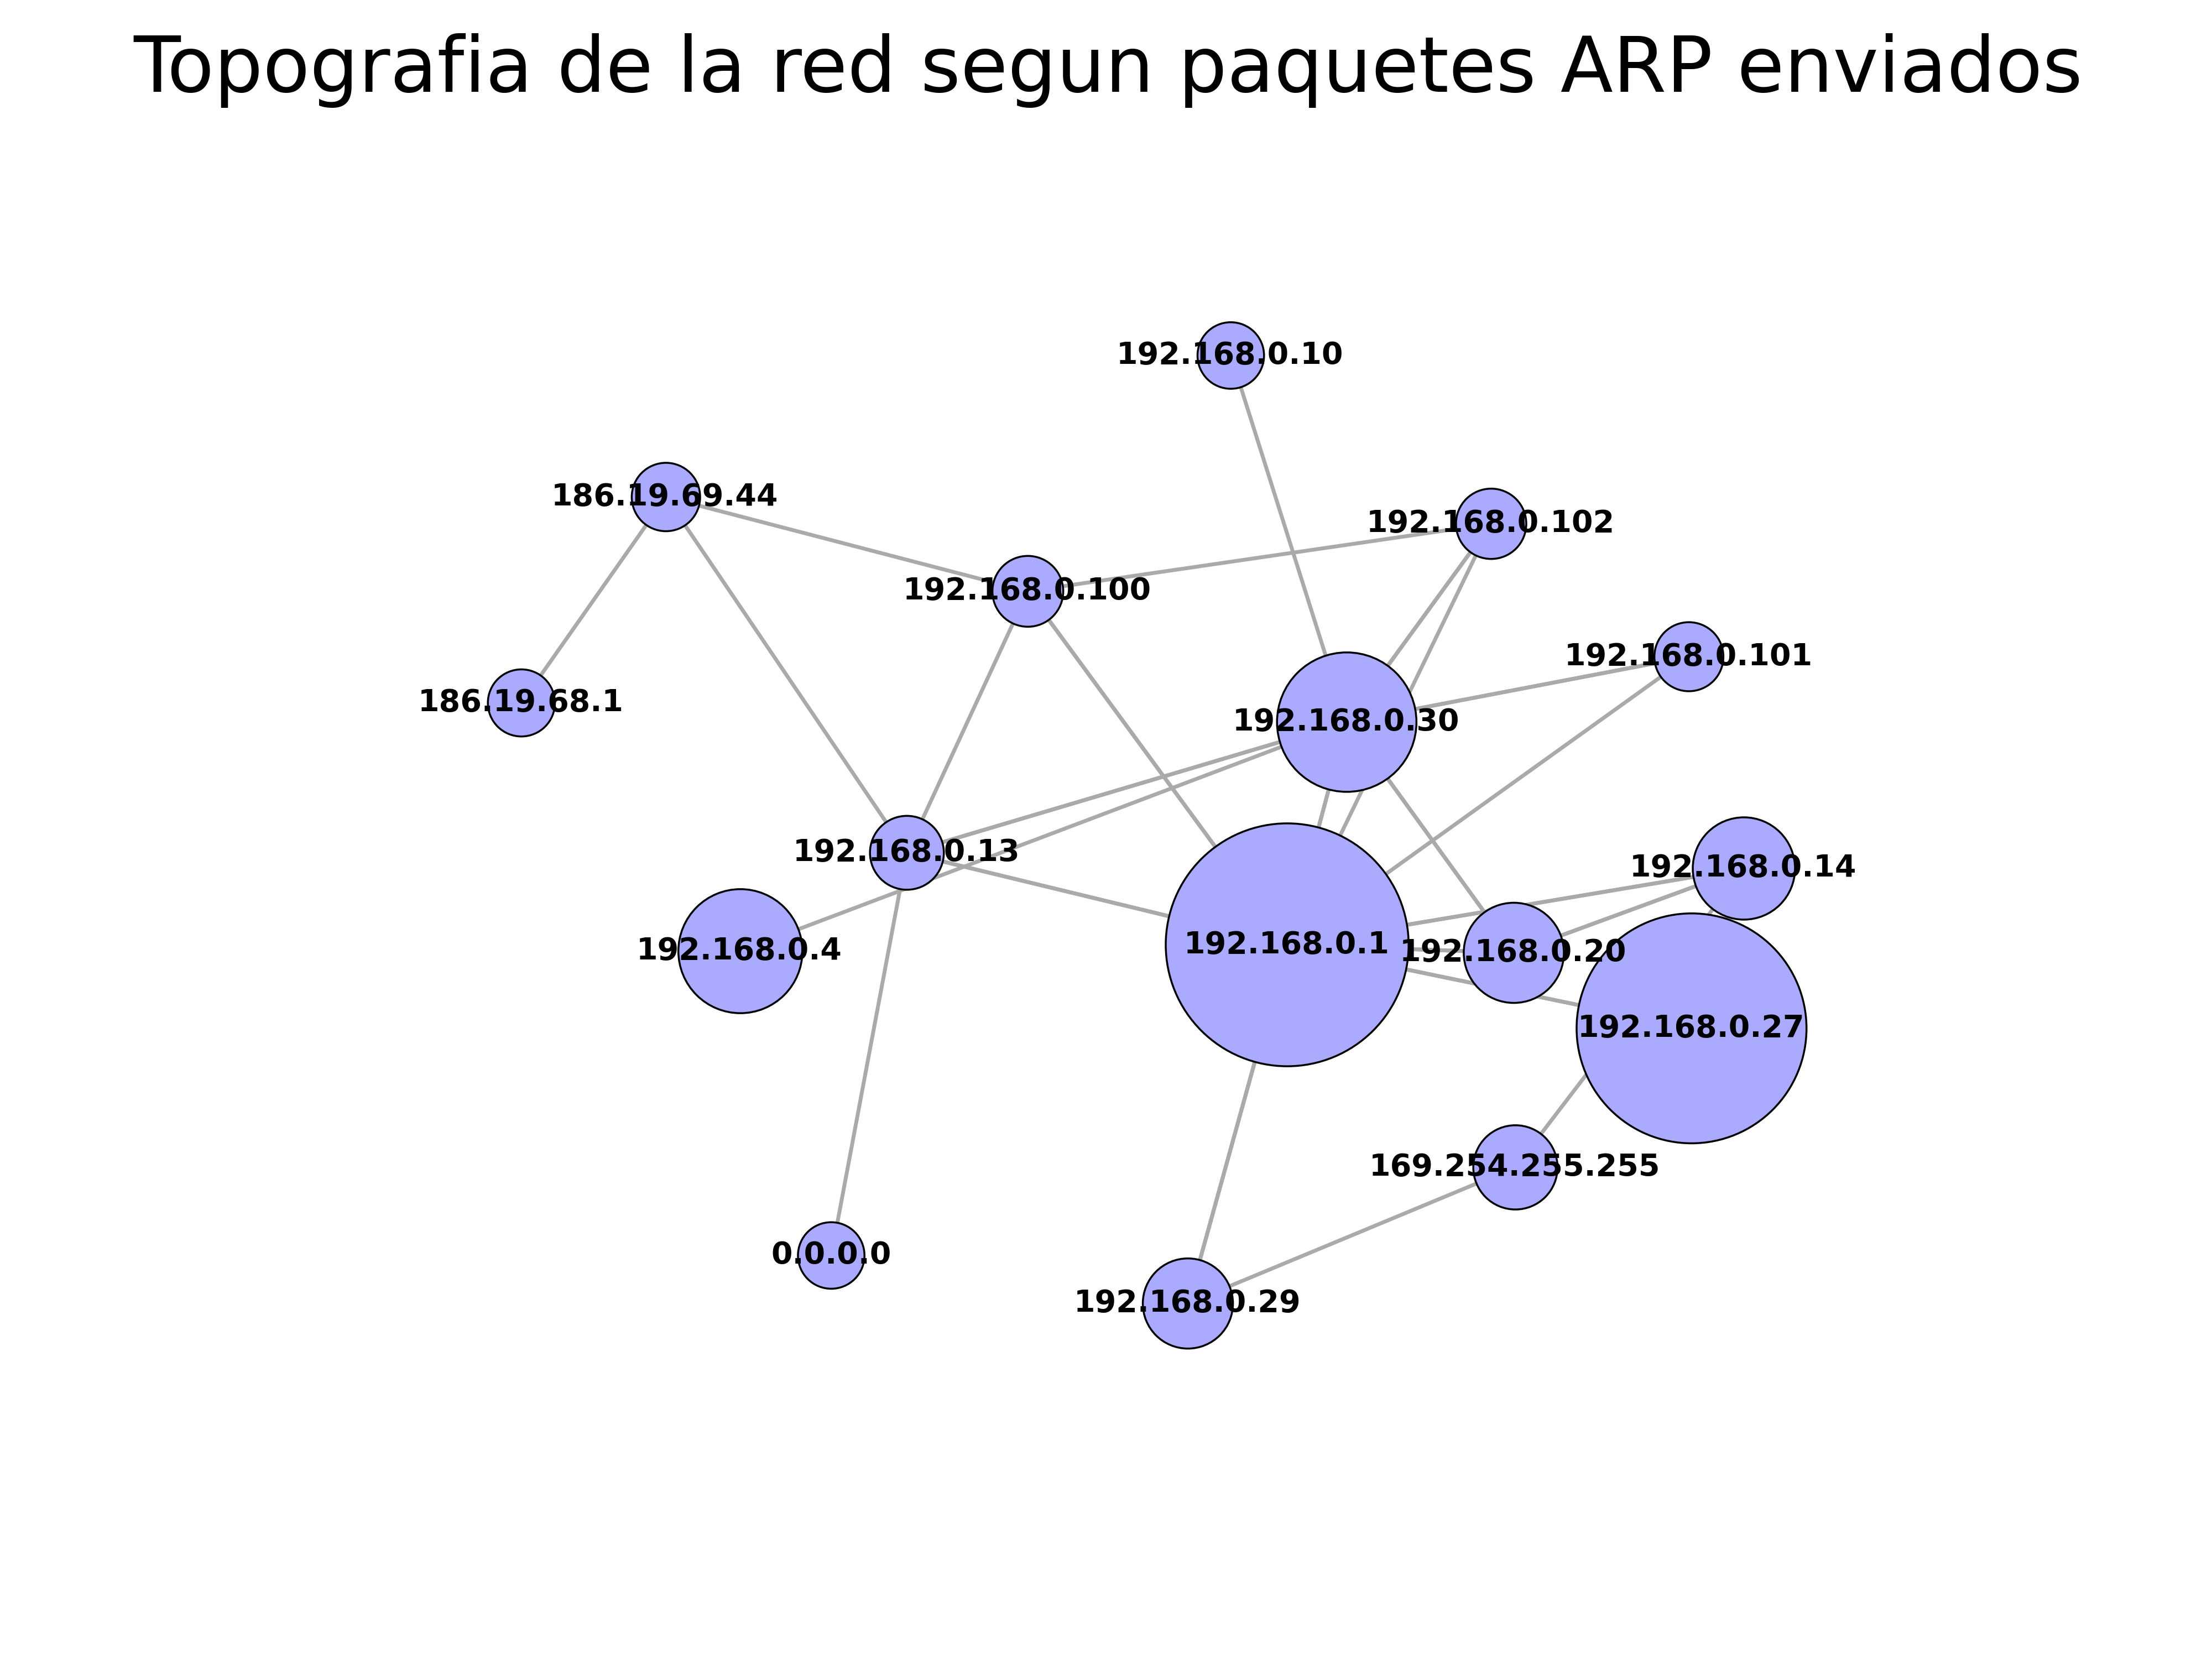
\includegraphics[width=0.7\textwidth]{graficos/red_domestica_network.png}
  \caption{Mi Figura}
  \label{fig:red_domestica_network}
\end{figure}

\FloatBarrier

\subsubsection{Histogramas (de IPs y protocolos)}

\begin{figure}[h!]
  \centering
   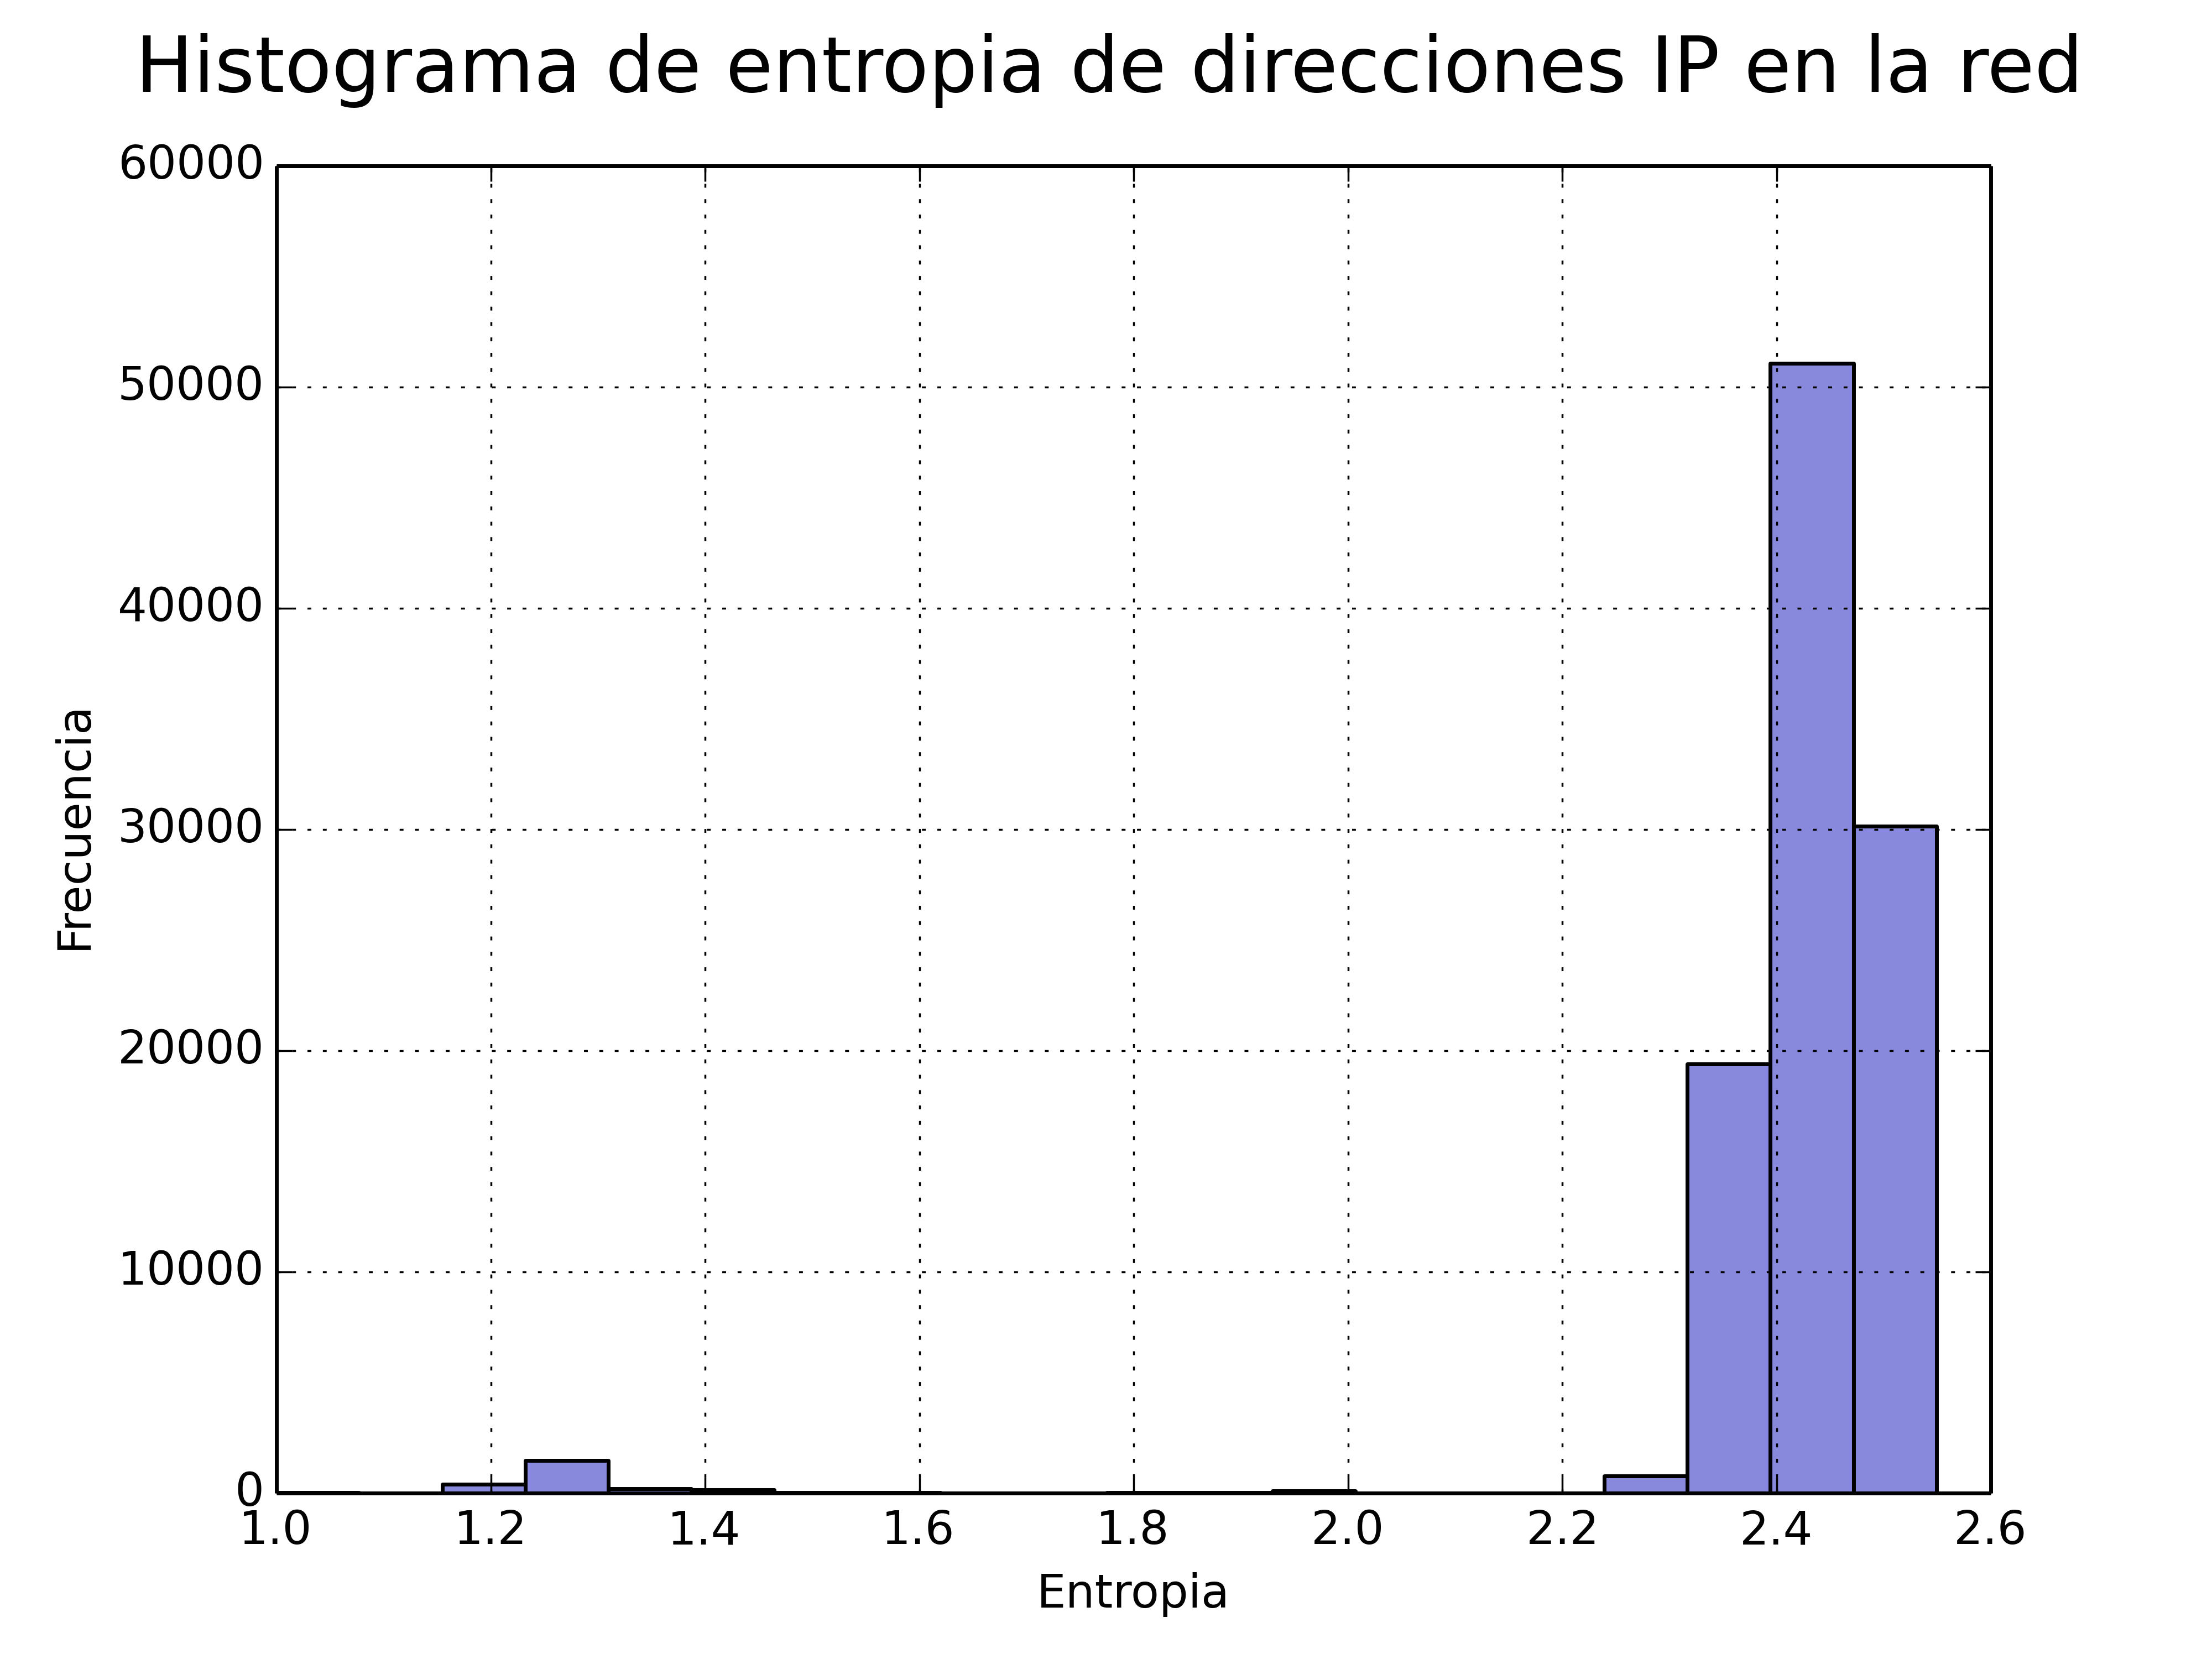
\includegraphics[width=0.7\textwidth]{graficos/red_domestica_hist_arp.png}
  \caption{Mi Figura}
  \label{fig:red_domestica_hist_arp}
\end{figure}

\begin{figure}[h!]
  \centering
   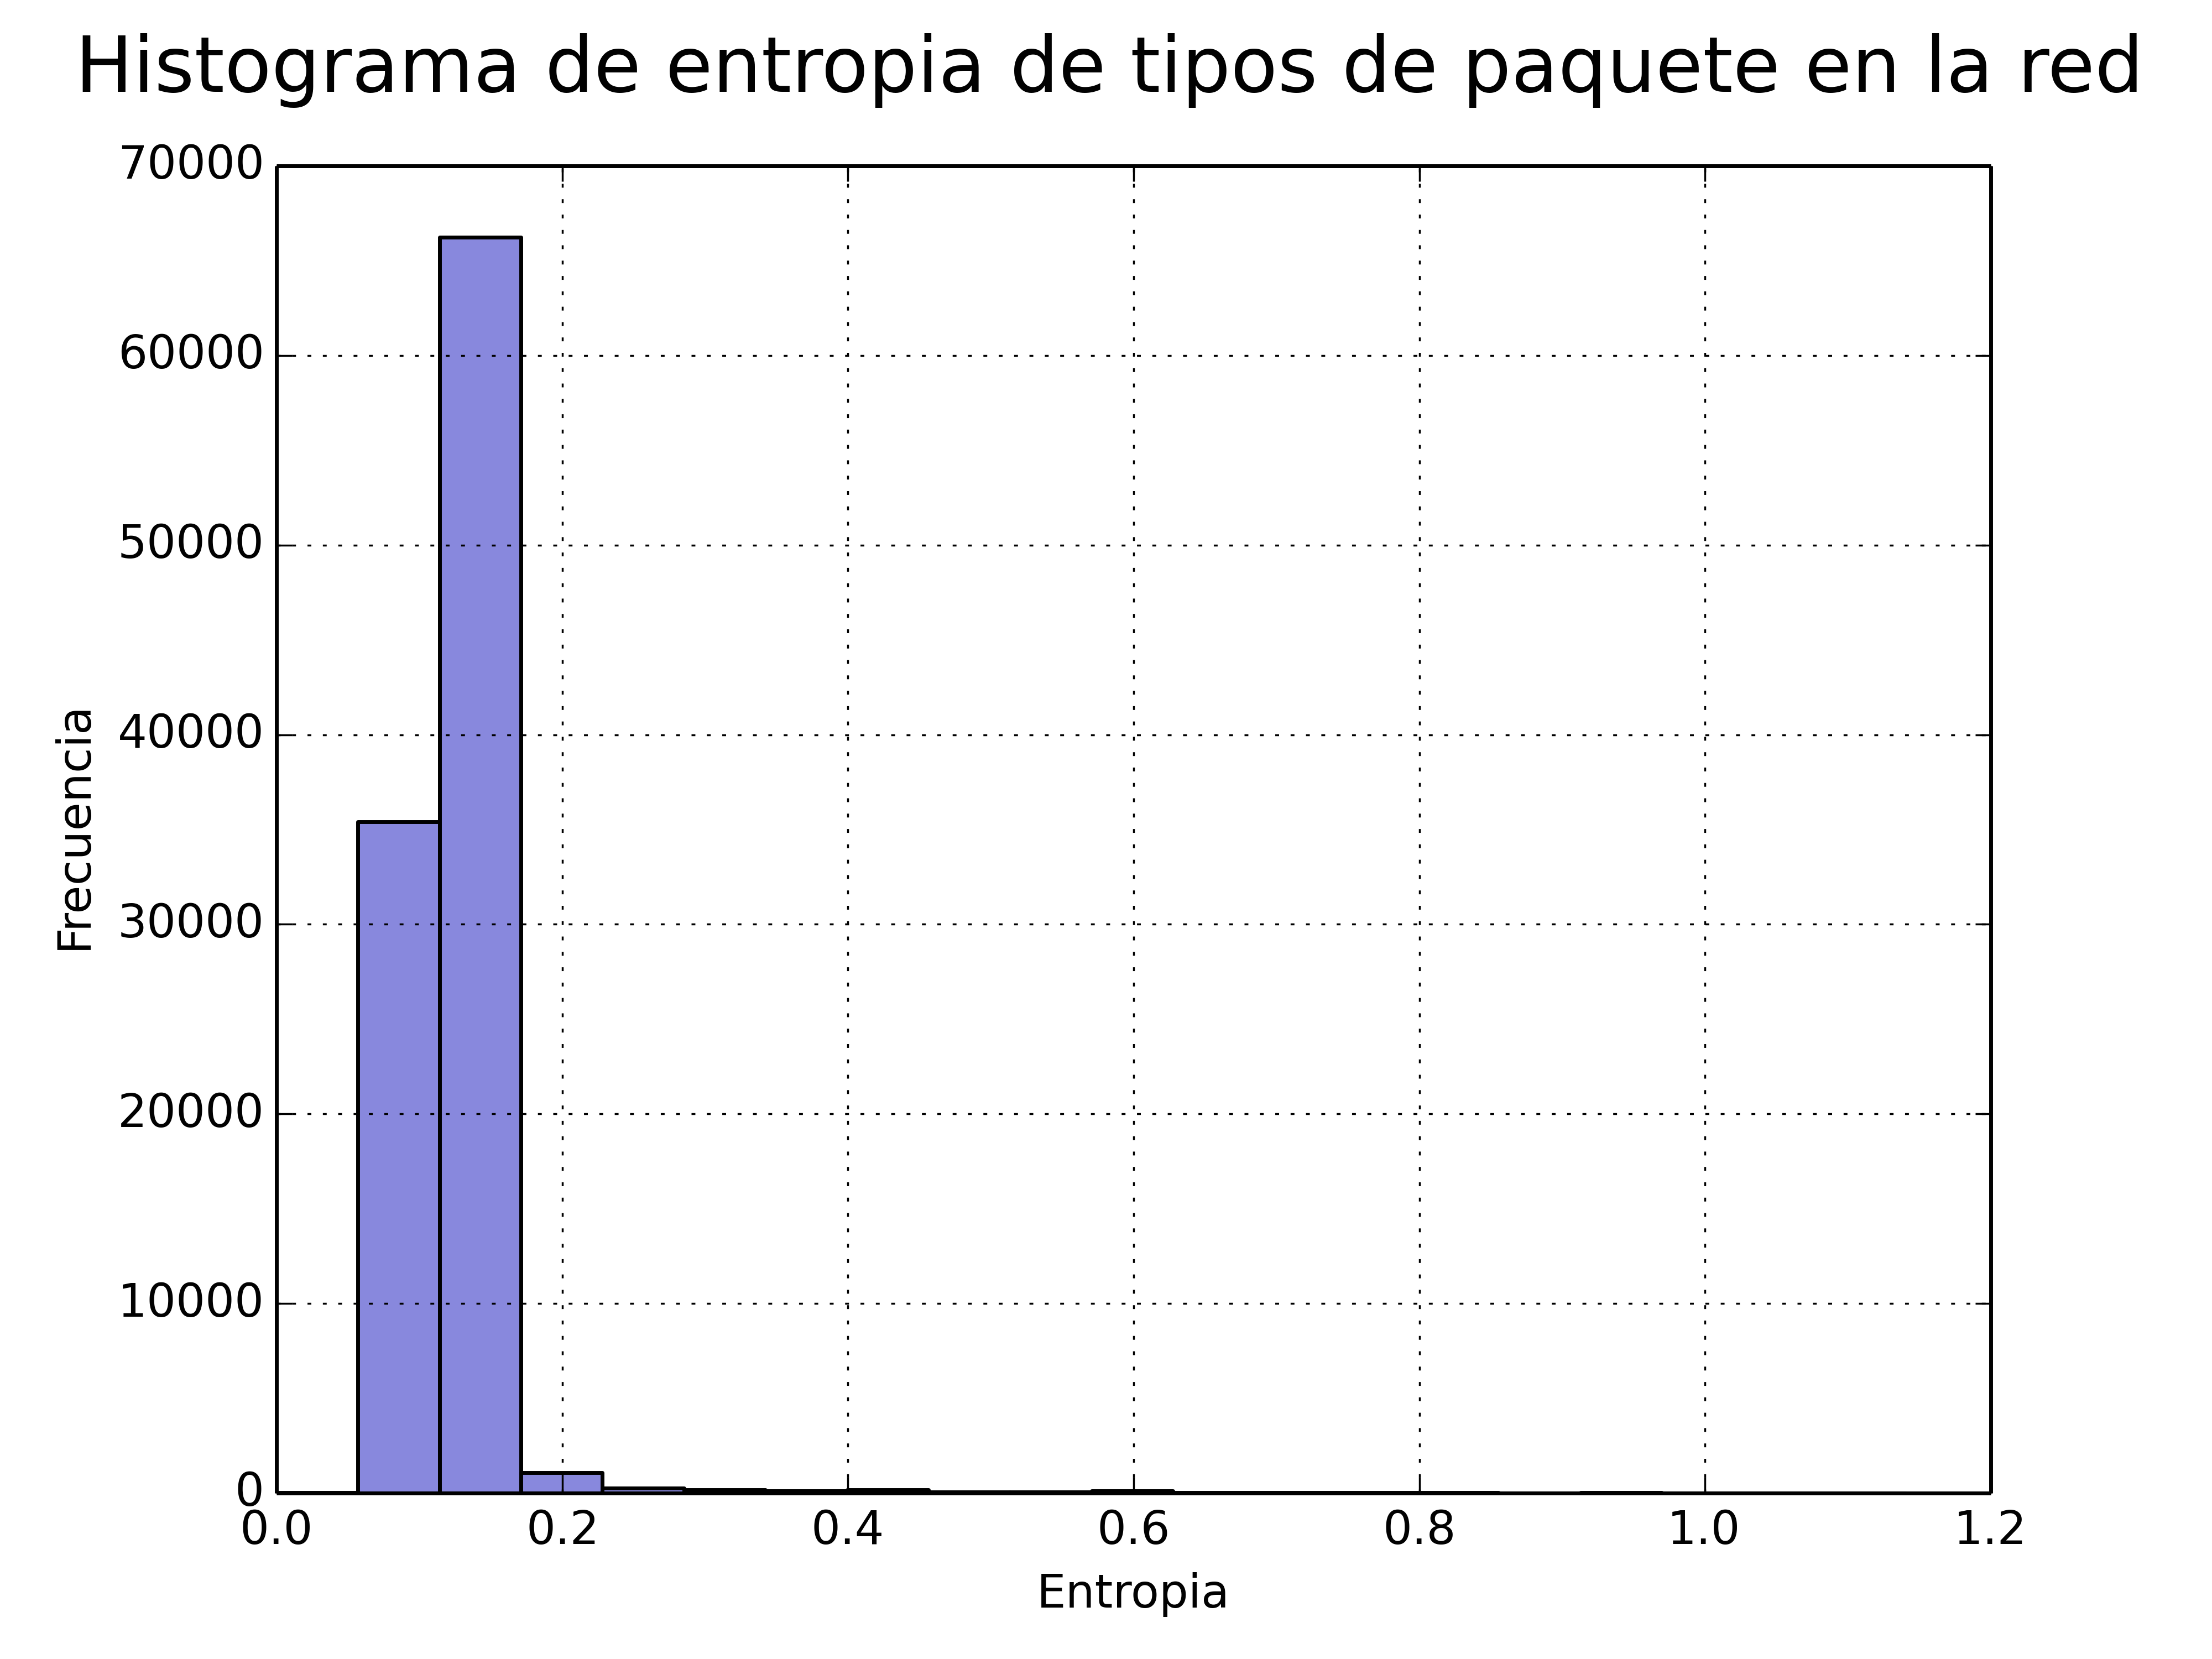
\includegraphics[width=0.7\textwidth]{graficos/red_domestica_hist_type.png}
  \caption{Mi Figura}
  \label{fig:red_domestica_hist_type}
\end{figure}

\FloatBarrier

\subsubsection{Paquetes capturados e información}

Los gráficos de torta, nos permiten ver la relación entre la cantidad de paquetes y la información que proveen cada nodo en la red. 
En los primeros 2 gráficos ~\ref{fig:red_domestica_pie_arp}. ~\ref{fig:red_domestica_pie_arp_information}. se toma como fuente las ips de la red.
Podemos notar que los nodos mencionados anteriormente son los mas frecuentes y por lo tanto los que menos información tienen.

En los siguientes 2 gráficos ~\ref{fig:red_domestica_pie_type}. ~\ref{fig:red_domestica_pie_type_information}. la fuente es la indicada en la cátedra. Vemos que el protocolo que mas se repite es el IP con un porcentaje muy superior al resto y aportando información casi nula. 

\begin{figure}[h!]
  \centering
   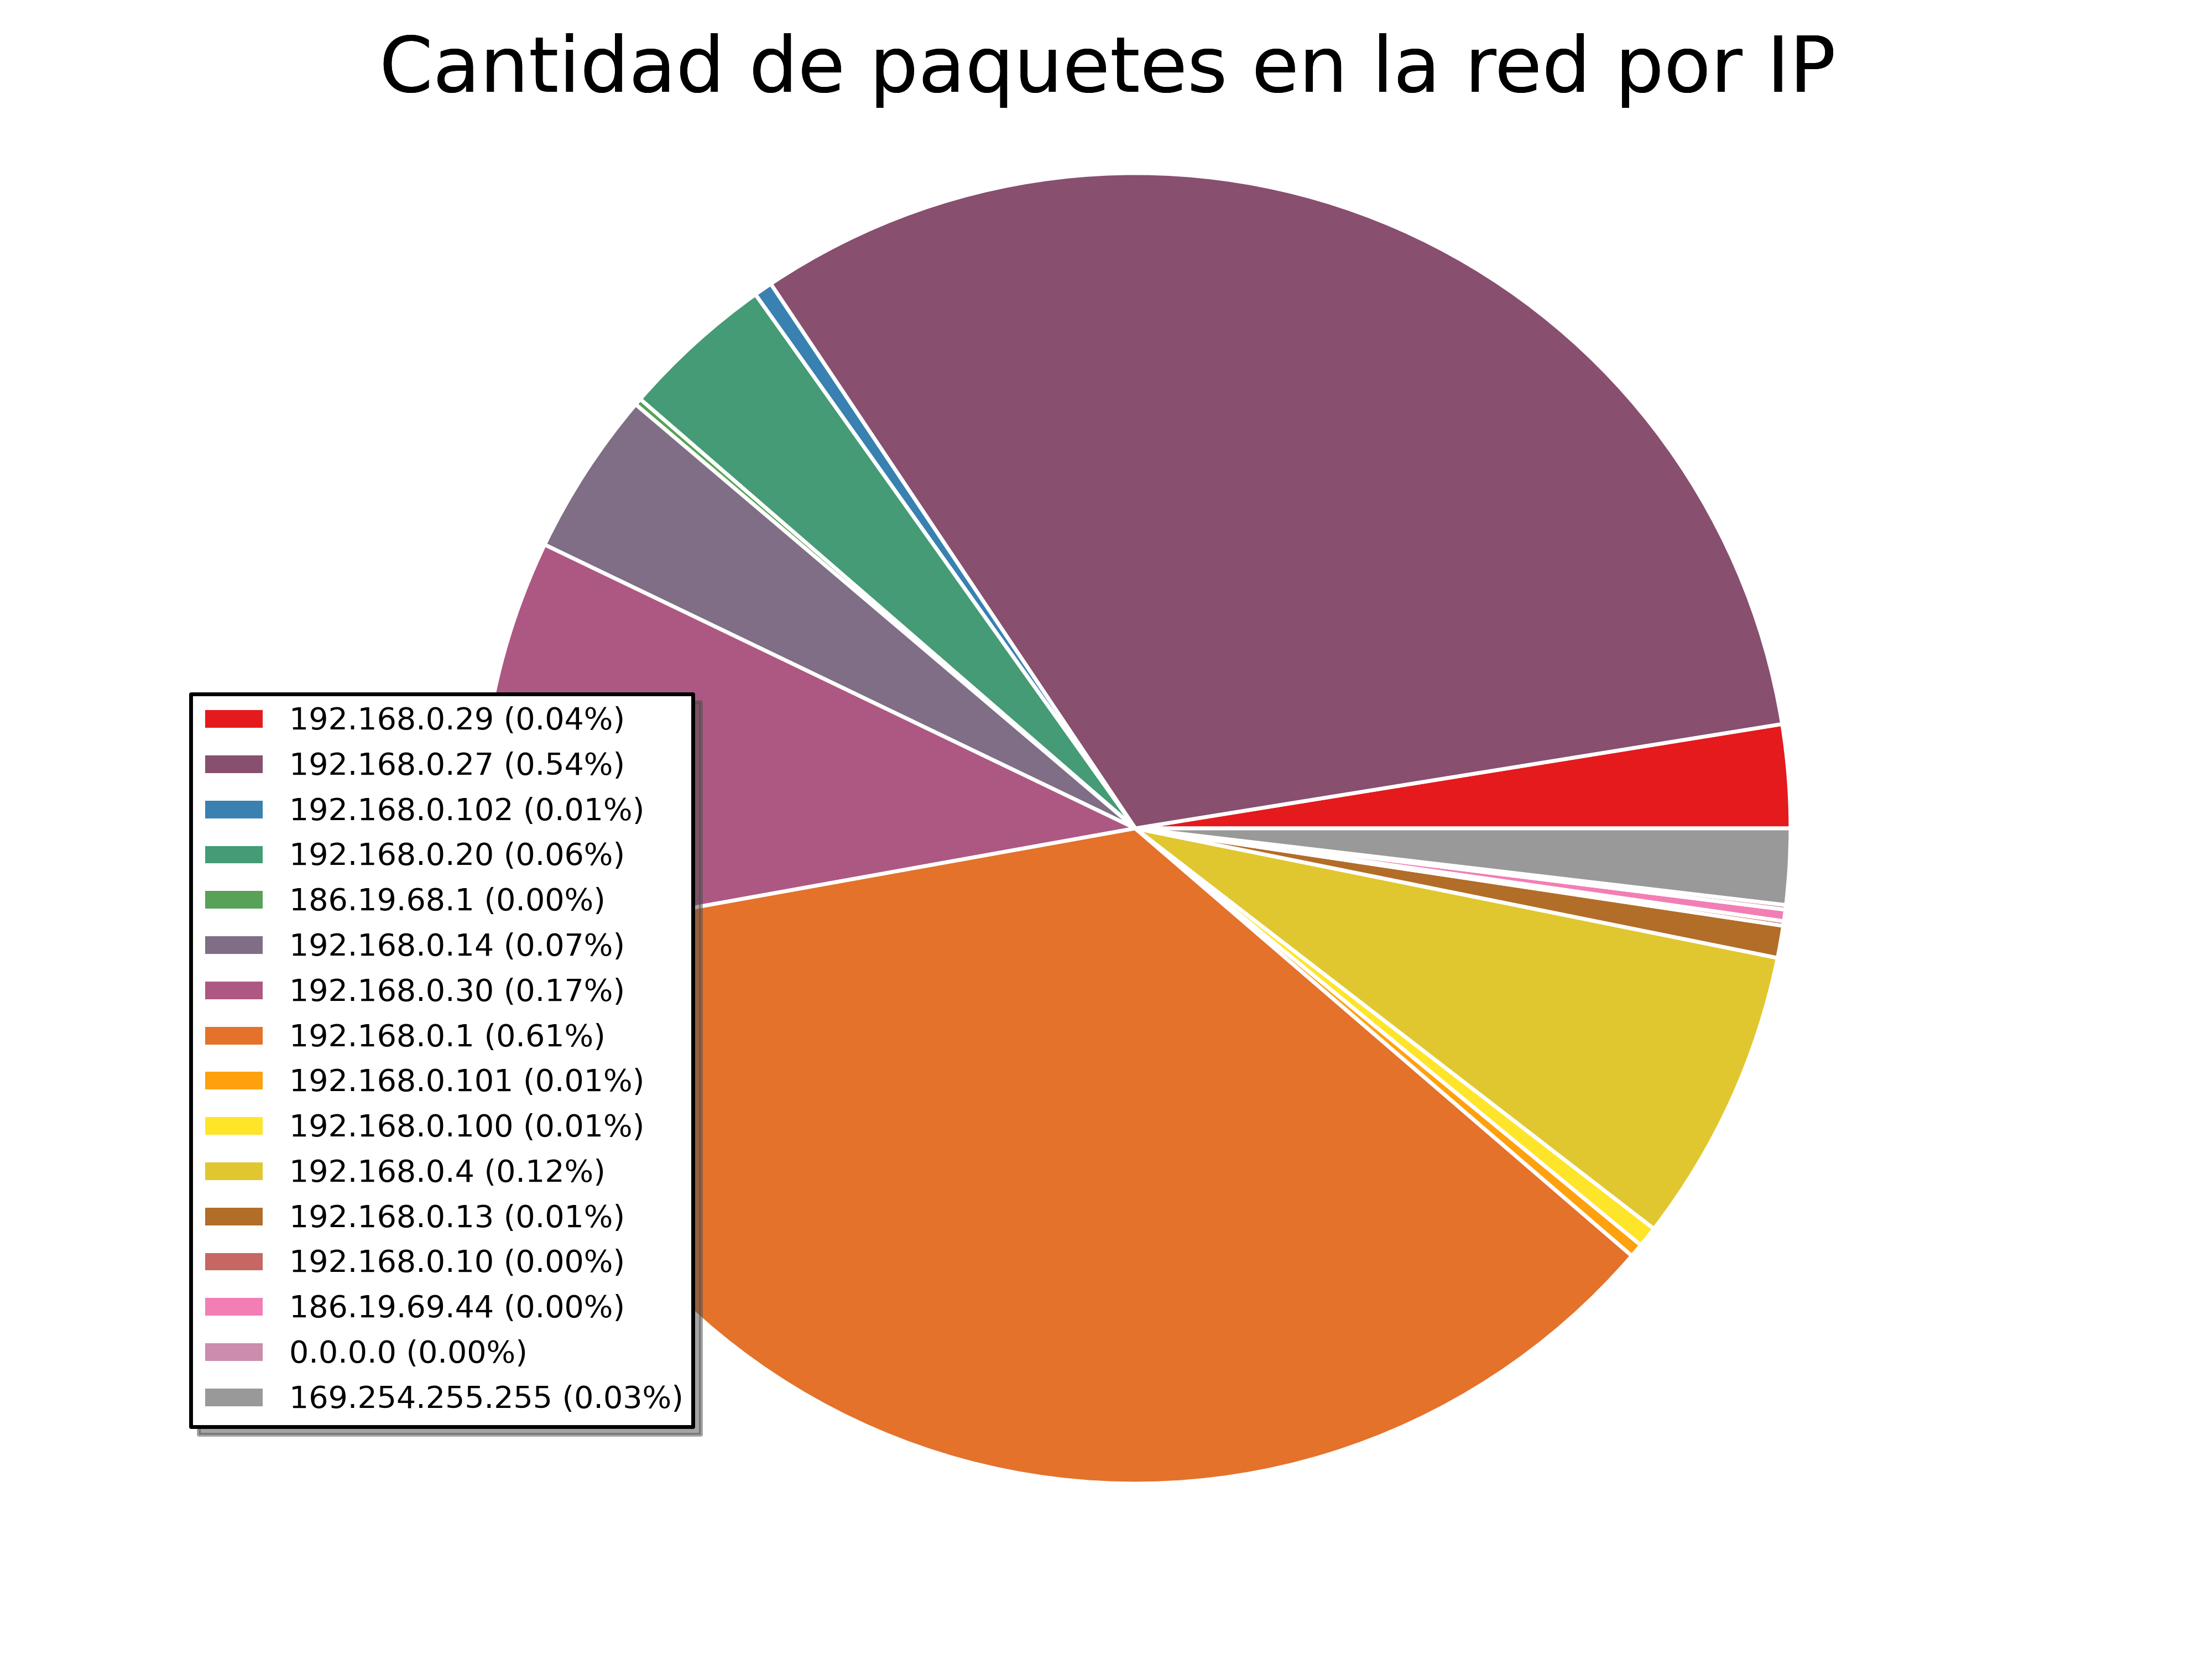
\includegraphics[width=0.7\textwidth]{graficos/red_domestica_pie_arp.png}
  \caption{Mi Figura}
  \label{fig:red_domestica_pie_arp}
\end{figure}

\begin{figure}[h!]
  \centering
   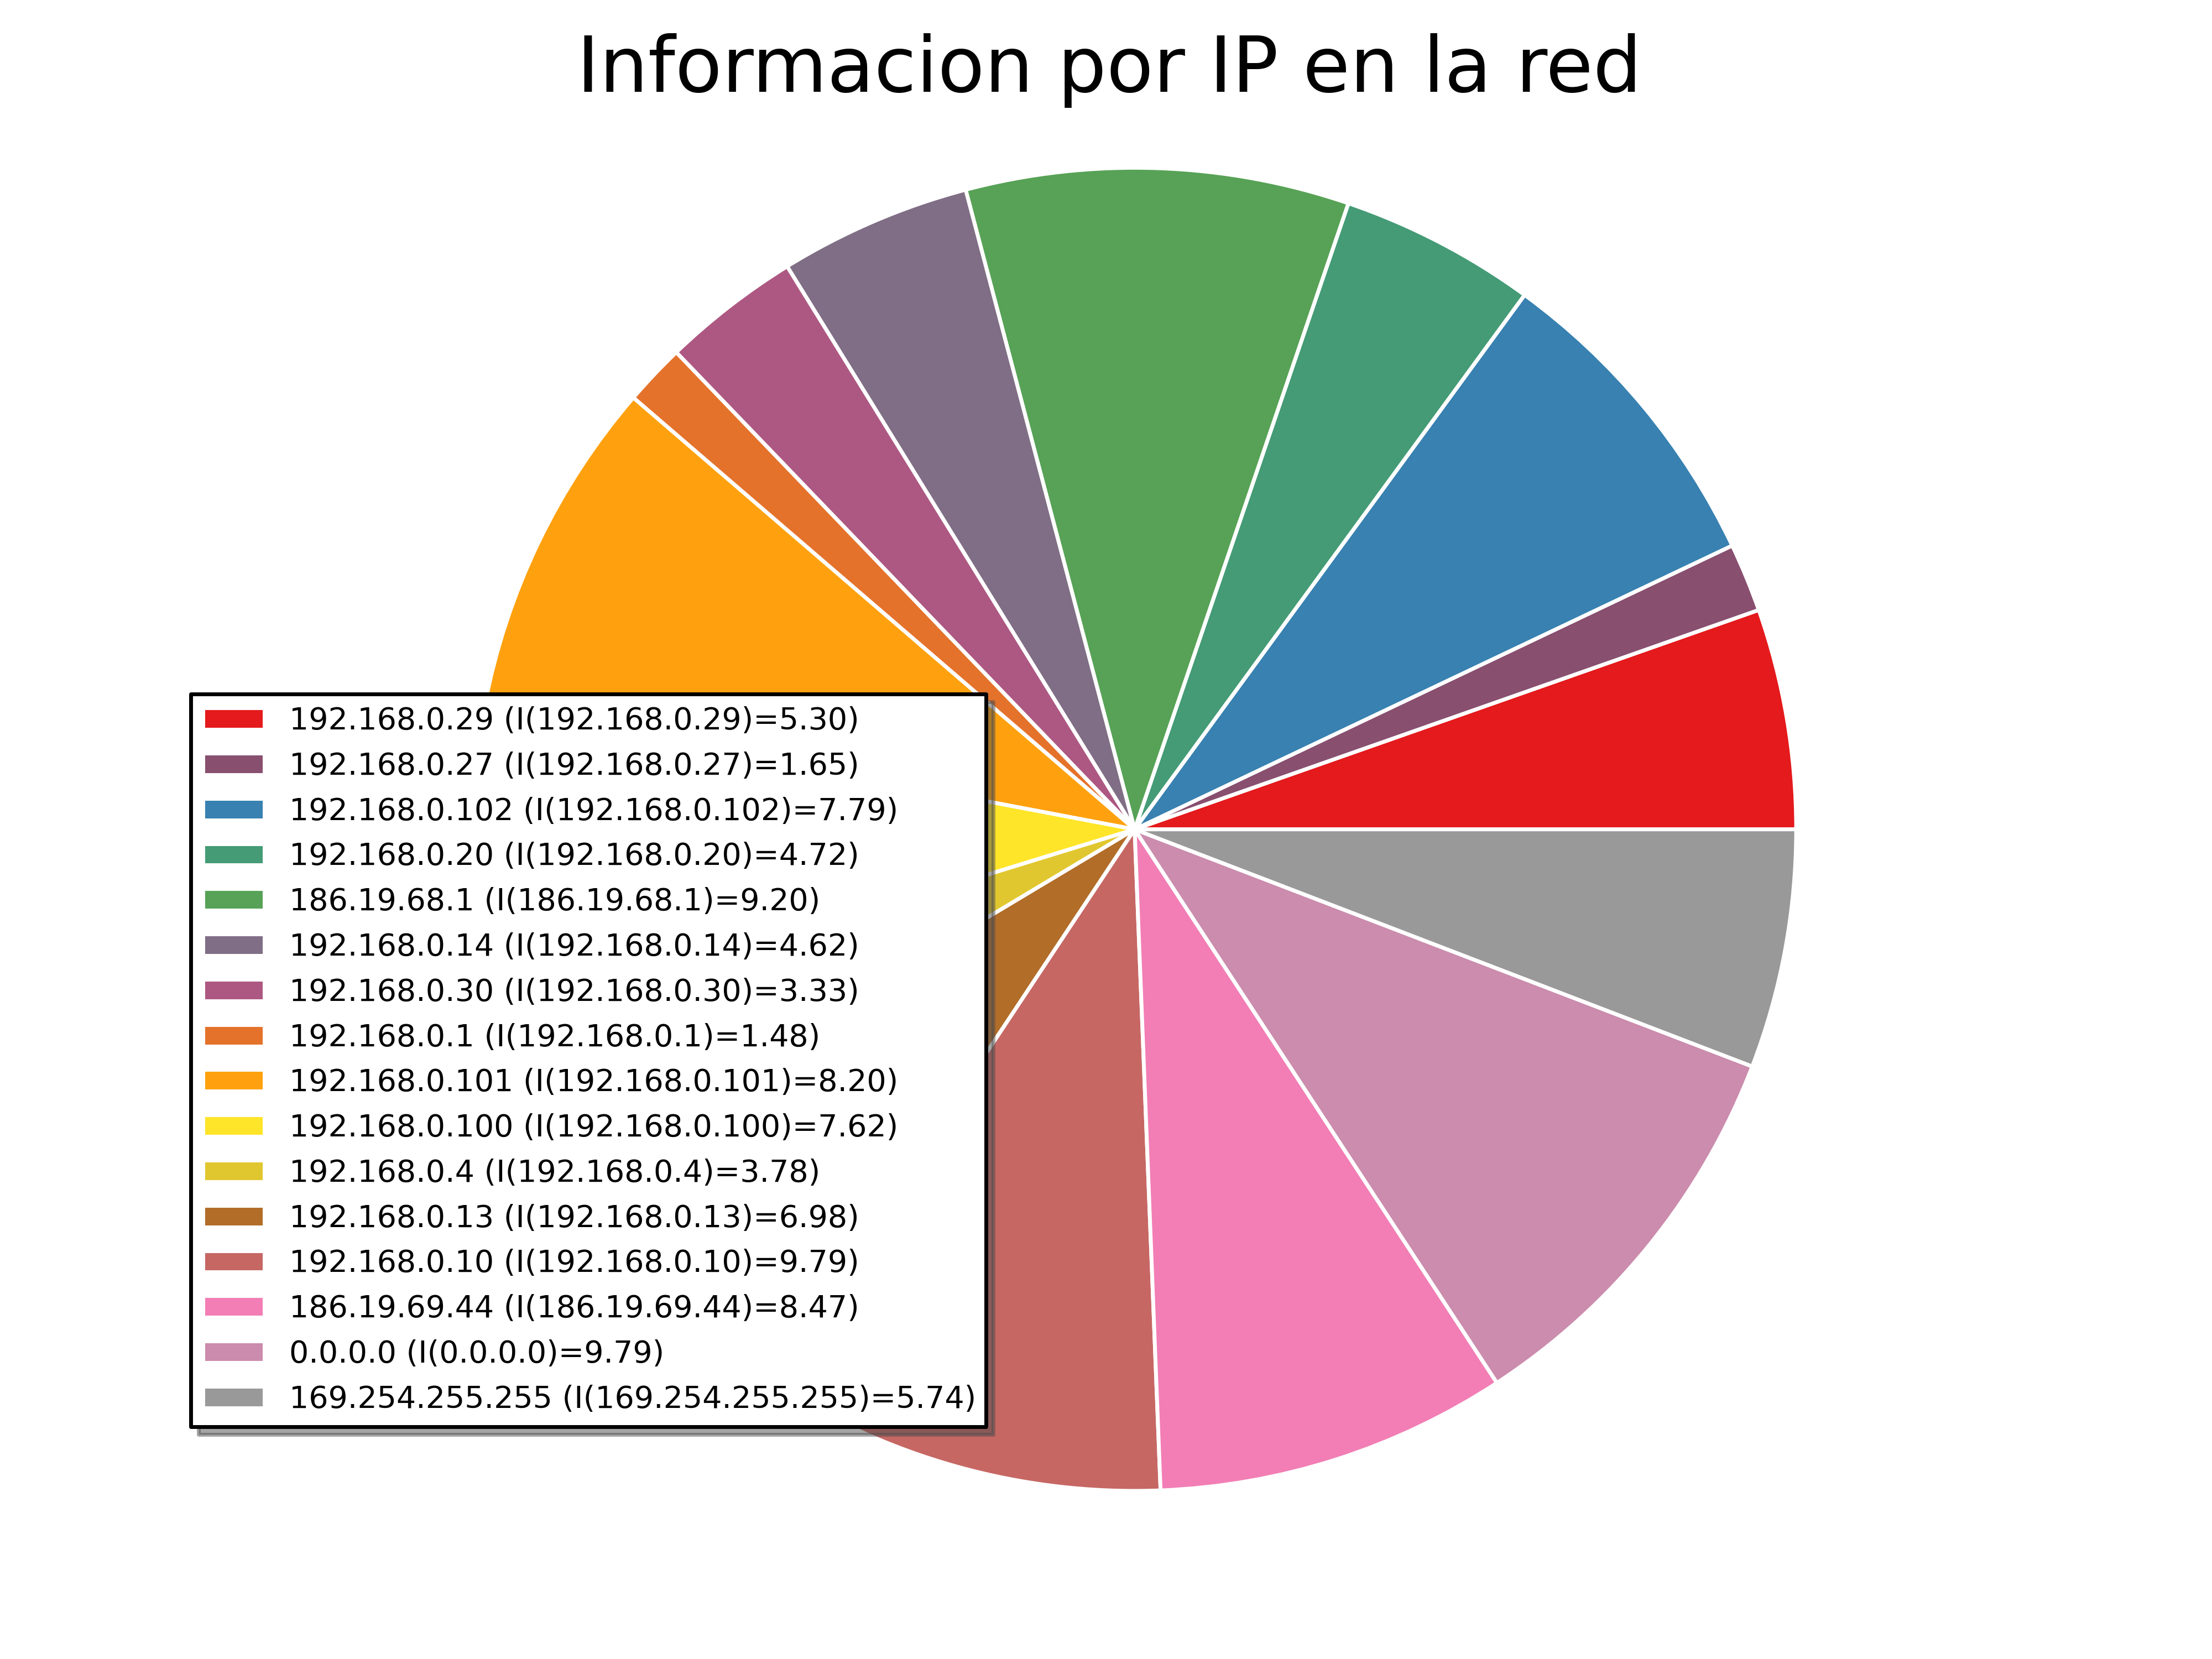
\includegraphics[width=0.7\textwidth]{graficos/red_domestica_pie_arp_information.png}
  \caption{Mi Figura}
  \label{fig:red_domestica_pie_arp_information}
\end{figure}

\begin{figure}[h!]
  \centering
   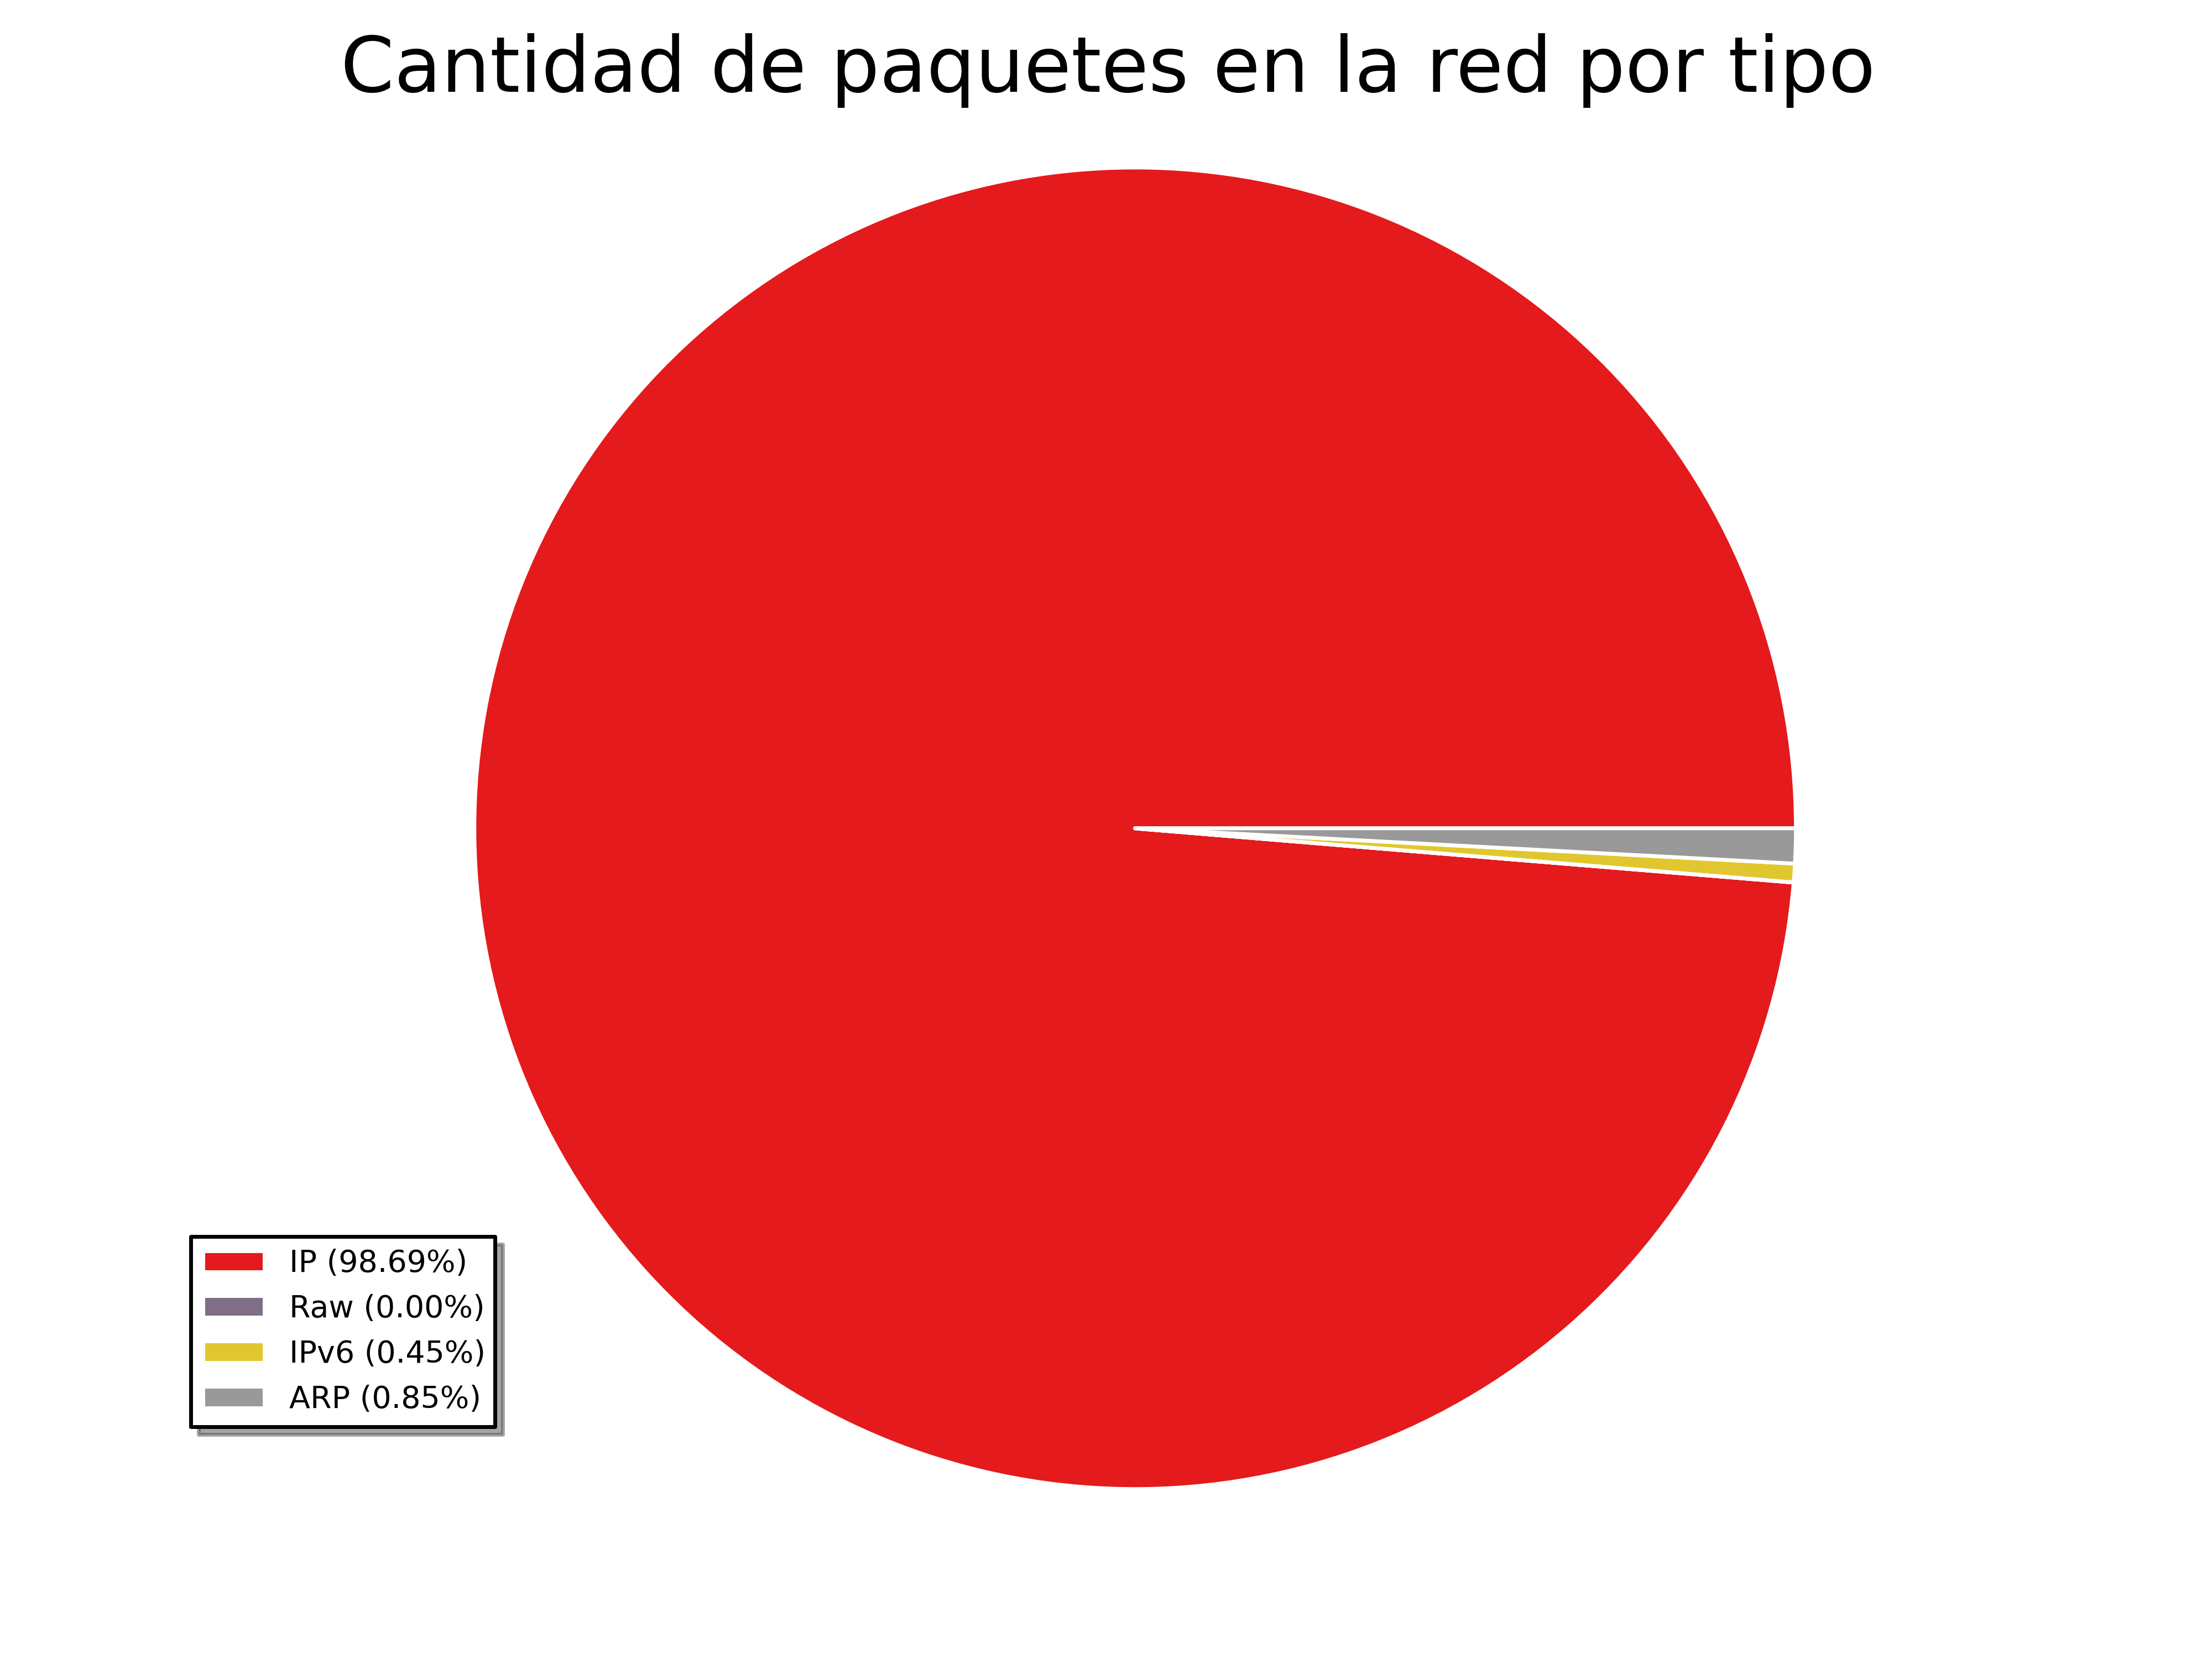
\includegraphics[width=0.7\textwidth]{graficos/red_domestica_pie_type.png}
  \caption{Mi Figura}
  \label{fig:red_domestica_pie_type}
\end{figure}

\begin{figure}[h!]
  \centering
   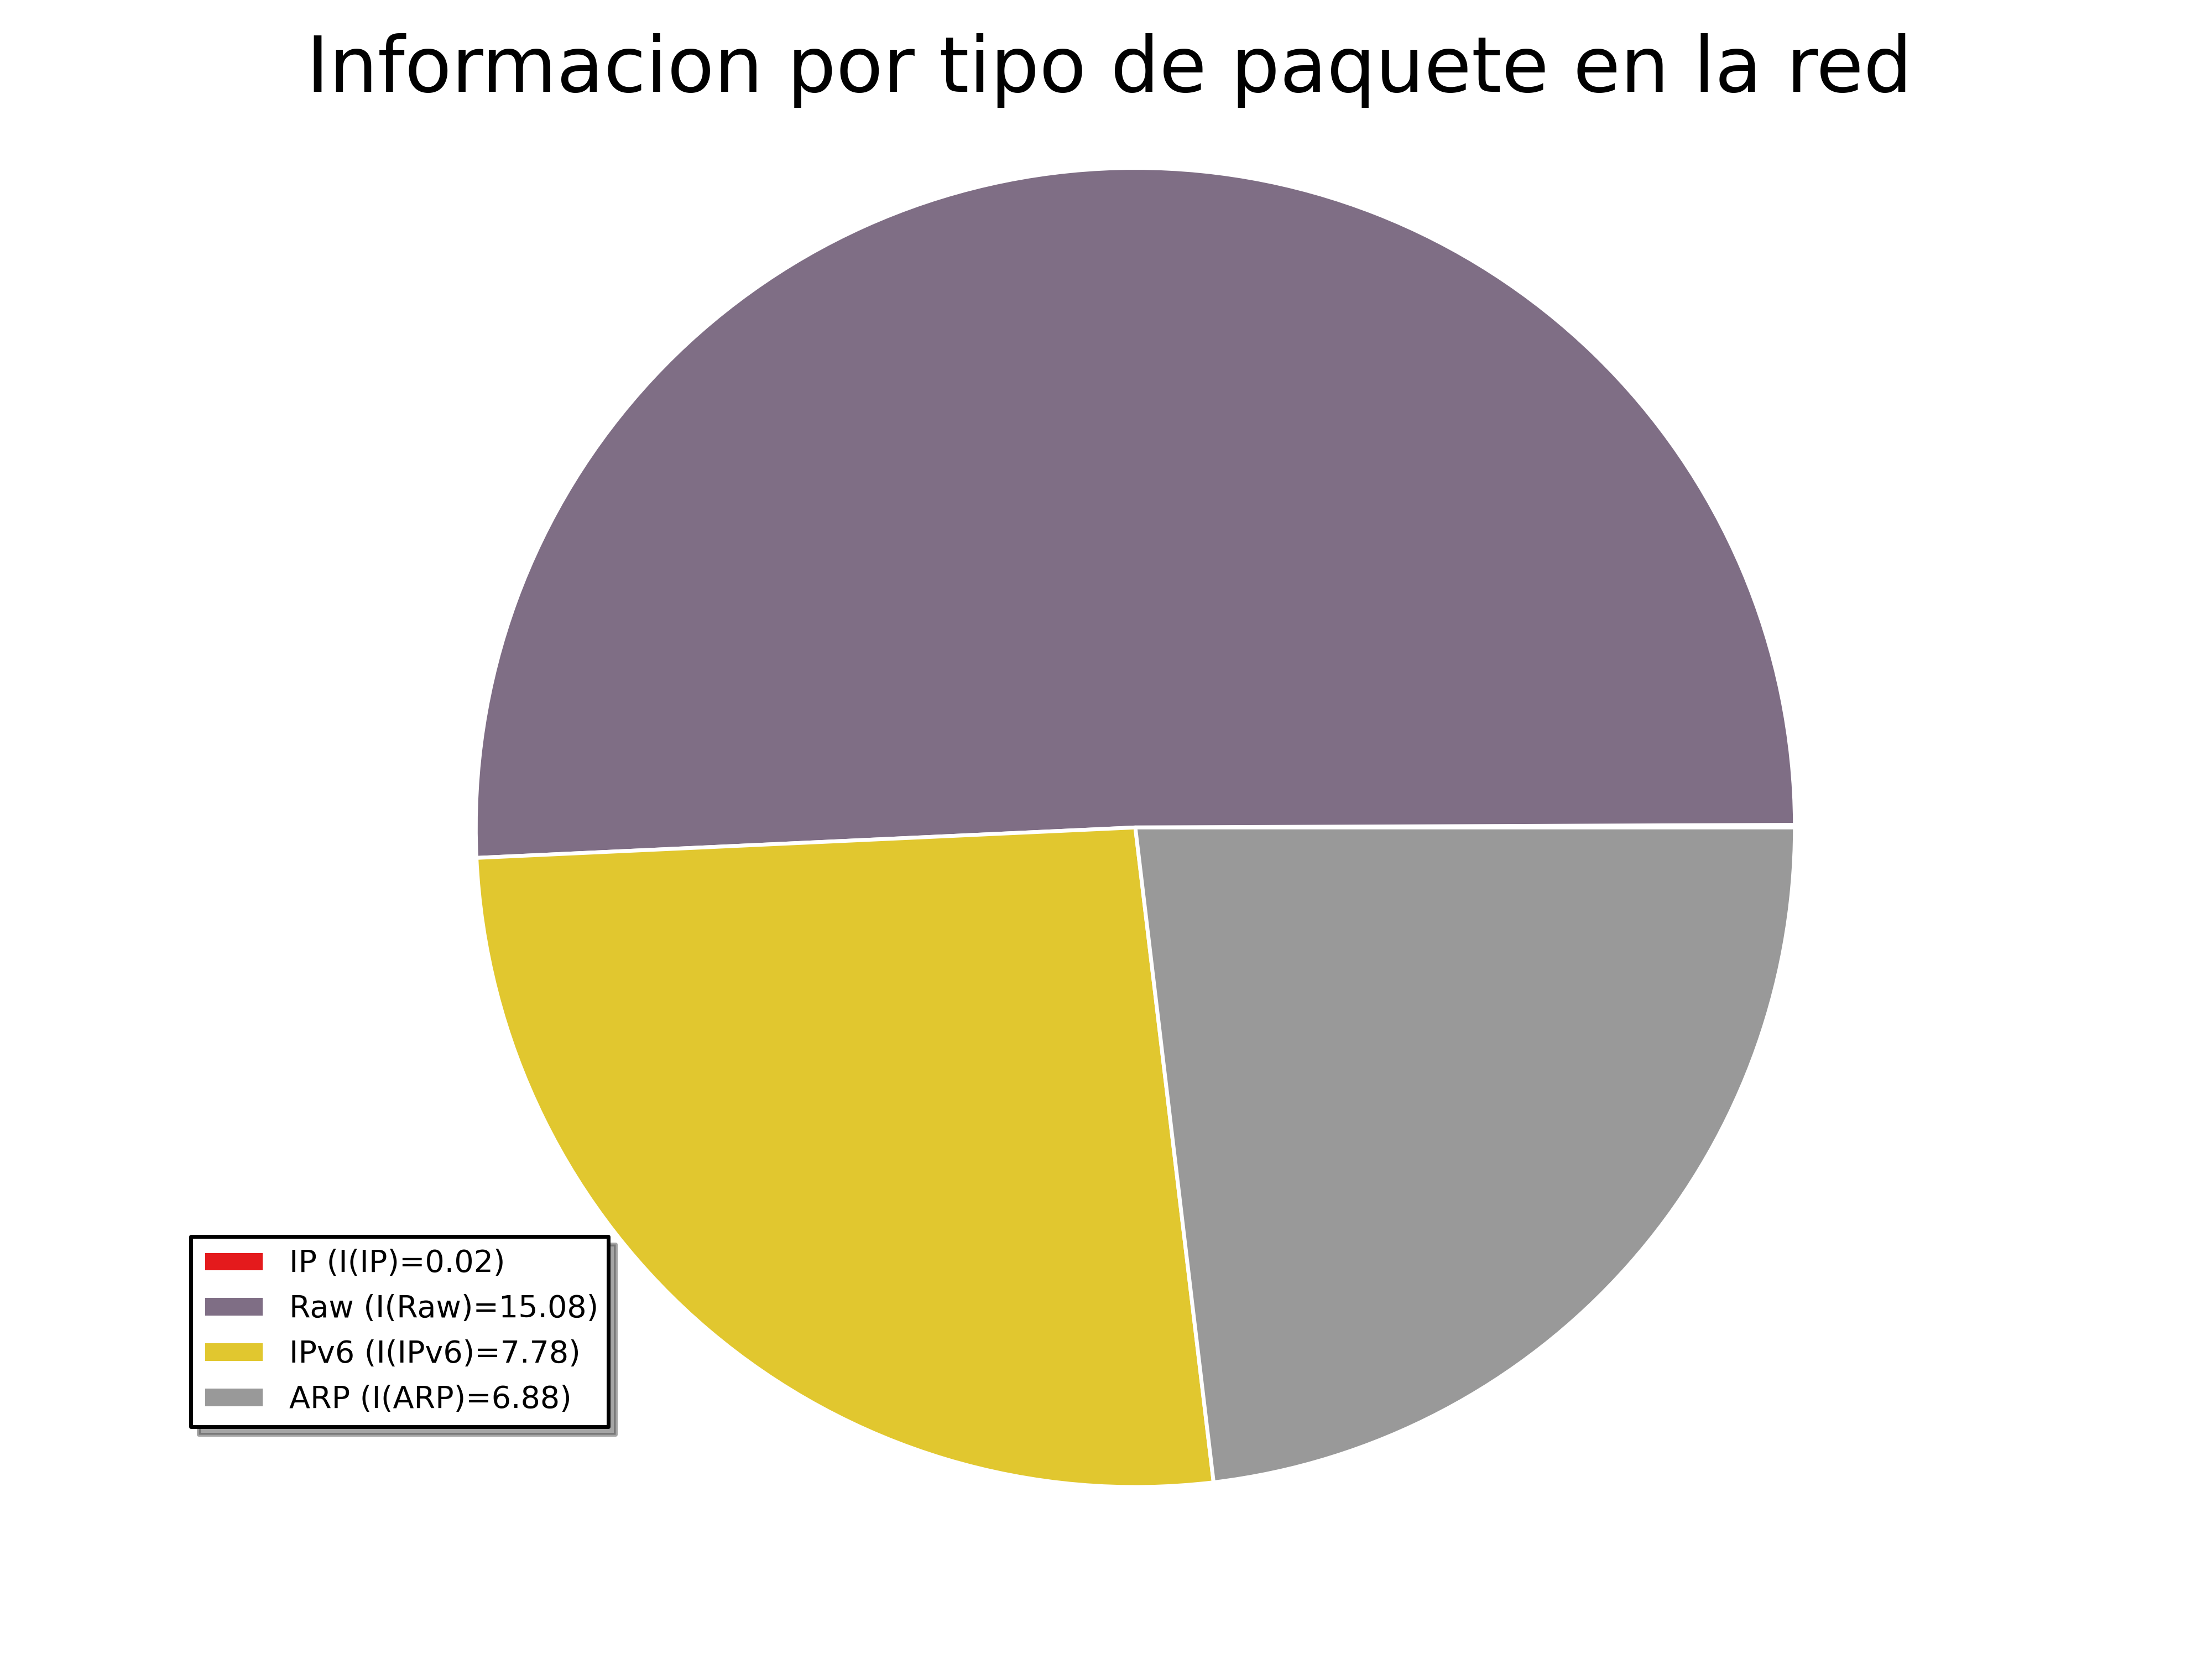
\includegraphics[width=0.7\textwidth]{graficos/red_domestica_pie_type_information.png}
  \caption{Mi Figura}
  \label{fig:red_domestica_pie_type_information}
\end{figure}
\pagebreak
\section{Conclusiones}
En estos experimentos pudimos apreciar una aplicación concreta de la teoría de la información que nos permitió modelar y analizar diferentes fuentes de información.
\\\\
En la primera parte del trabajo práctico, al buscar protocolos distinguidos se descubrió que, en general, el protocolo más frecuente es el IPv4, lo cual es razonable. Además se notó que en algunas redes el protocolo IPv6, también, es bastante frecuente y que el protocolo ARP siempre se encontró presente en ellas. Esto último es previsible, por el funcionamiento de las redes IP en LAN.
\\\\
En el análisis de protocolos pudimos encontrar muchas similitudes entre las distintas redes. En general la entropía de esta fuente presentó un valor bajo y además el protocolo IPv4, que es el que mayor tráfico presenta, aportó valores de información inferiores. Esto demuestra una fuente predecible en la que se espera que la mayoría de los paquetes pertenezcan al protocolo IPv4.
\\\\
En la segunda parte del trabajo se investigó la existencia de nodos distinguidos (o símbolos distinguidos en el contexto de la fuente $S_1$).
\\\\
Se pudo observar que en las redes analizadas el router fue uno de los nodos distinguidos.
\\\\
También se observó que para las fuentes que modelan los diferentes nodos de la red, el valor de la entropía fue más elevado que la entropía de las fuentes que modelan los tipos de protocolos. Esto nos parece razonable debido a la impredecibilidad de la incidencia de los nodos en la red en comparación con la de los diferentes tipos de protocolos.





%\newpage
%\begin{thebibliography}{9}
 %\end{thebibliography}


\end{document}

